
\documentclass[11pt,a4paper]{report}
\usepackage[utf8]{inputenc}
\usepackage[a4paper]{geometry}
\usepackage{graphicx}
\usepackage{listings}
\usepackage[dvipsnames]{xcolor}
\usepackage{tikz}

\usepackage{CrimsonPro}
\usepackage[T1]{fontenc}
%% The font package uses mweights.sty which has som issues with the
%% \normalfont command. The following two lines fixes this issue.
\let\oldnormalfont\normalfont
\def\normalfont{\oldnormalfont\mdseries}

\title{Image compression: On-demand systems seeking minimal latency.}
\author{Kobe Vrijsen}
%\date{January 2023}

\begin{document}
\pagenumbering{gobble}

\maketitle

\begin{abstract}

Latency and loading times in on-demand settings such as web pages and network streaming and how to minimise it. Image downloads generally take up a large portion of loading times and this paper will discuss and test several methods and formats that aid to reduce latency. Analysing variable factors and their effects on loading times. Discussing both common formats, including PNG, Webp and JPEG, as well as lesser-known compressors like Qlic. Is there an excelling format or does it differ on a per use case basis. This paper aims to provide insight and hopes to assist making choices regarding image compression and how to use it.

\begin{center}
    \item \paragraph{Keywords} Image compression, Image formats, Latency, Loading times, Web pages.
\end{center}
\end{abstract}


\newpage

\tableofcontents

%\newpage
%\chapter*{Preface}
%A bachelor programme research. 
%Preface text

\newpage
\pagenumbering{arabic}

\chapter{Introduction}

%A primary goal of optimising applications for mobile devices is minimising loading times and latency. While network latency and carriage capacity is not something that the game, client or server can reasonably do something about, the amount of queries and data requested can be adjusted and optimised. Requesting less data less frequently can result in a faster overall response time and better experience.

On-demand systems seeking minimal latency. Time is key, specifically as little of it as possible. Can image compression be utilised to improve client-side latency? If so, what factors play part and which method offers the best solution? Or is it perhaps determined by its use case?

How compression affects performance as well as overall loading times will be the main focus of this paper. If compression is beneficial, what factors need to be taken care of and kept in mind to get to the best possible solution for our system?

\section{The system}

\subsection{On-demand systems}

Web pages, network streams, games, chats rooms, the list goes on. All are examples of systems that are, either in part or in full on-demand systems. What defines an on demand system is that resources to be requested are unknown before before they are requested. As soon as it is required or has to be shown, a request must be sent out which is responded to with the necessary data. This is the basic concept of on-demand systems. The time it takes from request to result is the heart of the experience. Every tool in the pipeline can be a potential bottleneck. This paper will focus on the data requested and how to provide an optimal solution to reduce the overall latency to a minimum at the best of our abilities.

\subsection{Images}

Continuing on the request data. Two-dimensional graphical raster data will be the focus from here on out: I.e. images, photos and textures. Images, as they will be referred to, commonly take up large portions of overall requested data. This is dues to their large quantity data required to correctly reproduce all details. A raw image can easily reach tens of megabytes. Compared to other request data, which do not often exceed the megabyte mark, images are very much in need of data saving measures.

One does not have to look far, there's already an uncountable amount methods and formats that are used or have been proposed. Some have been useless, others have brought improvements, while some have set a true precedent going beyond what was previously thought possible. It has become a rather rare occurrence for any person to encounter a normal raw image. Image compression has become trivial enough for it to be a fair waste to not make use of it.

\subsection{Requests}

A request is made with the goal to ultimately receive a response. While for may years in human history severely slow and lossy mouth to mouth communication had been all there was, in this day and age there is a strong sentiment for requests to be as close to instantaneous as possible while transmitting the response in a perfectly intact state.

Firstly a request is sent out over a network, before a response is received there is a moment of silence. Neither light travels instantaneous nor will our data. This term is referred to as network latency or response time. From a client's perspective, this can unfortunately not be changed. Because of this the frame of reference in this paper will begin at the time the first glimpse of the response is received.

Next, the response will carry data that is not of no size. It will take time to receive the full response. This time is determined by the capability of the network, called the network bandwidth or speed, as well as the size of the total response size.

\subsection{Processing}

Data received from out response isn't just any data that can be copied straight to the screen. At least not when talking about compression. A compressed set of data has to be processed and inflated back to its original full sized content and possibly have some additional changes to its layout applied. This will inevitably take time. This may be referred to as processing time, decompression time, initialisation, loading time, etc. After the data transmission time itself, the download, this phase will most likely affect the final loading time, or latency, the most.

\section{Existing methods}

There are several methods of compression available. There's general compression algorithms that can be used as well as image specific compression algorithms. In the latter category there's also a distinction between lossless and lossy compression. As opposed to lossless, lossy compression results in a reduction of detail.

\subsection{No compression}

There are several formats used to save images that do not apply compression at all. Each one may have its reasons to do so. A few are listed below but will not be included in the benchmark. They will, however, serve as source files instead for our test cases.

\subparagraph{PPM}

Portable Pixmap Format, PPM \cite{ppm}. An extremely simple format saving essentially only the raster size and pixel data.

\subparagraph{BMP}

A simple format to store bitmap data \cite{bmp}.

\subsection{General compression}

General compression algorithms focus on compressing any kind of binary data. While not optimised for images, this does not hinder their ability to do so. In fact, formats like GIF, PNG and more formats than one might expect all default to this method internally. To get a frame of reference against image specific compression algorithms, the following algorithms will also be included in the benchmark:
 
\subparagraph{LZ77}

Lempel-Ziv \cite{LZ77}. Commonly referred to as Deflate. This is the default algorithm for containers like ZIP and and PNG. It is also often used to compress on-the-fly network streams. An old and all-round acceptable algorithm.

\subparagraph{LZMA}

Lempel–Ziv–Markov chain algorithm. Developed by the same author as the 7-zip compression tool \cite{7zip}. An extension of the default Lemper-Zif algorithm, it tries to improve compression by tweaking its values.

\subparagraph{GNU gzip}

A compression algorithm and tool created by the Free Software Foundation \cite{gzip}. Commonly used on Linux like operating systems and by developer communities. A common algorithm used to compress tarballs and also used to compress on-the-fly network streams.

\subparagraph{bzip2}

An implementation of the Burrows-Wheeler algorithm \cite{bzip2}.

\subparagraph{PPMd}

Prediction by Partial Matching. An implementation by Shkarin Dimitri \cite{ppmd}.

\subsection{Image compression}

Image compression comes in many forms. From general lossless compression to image specific lossy compression. Each with its own advantages and disadvantages. We'll mostly be discussing the  formats and algorithms commonly used on the web today as well as some up and coming algorithms with promising features.

\subsubsection{Web}

Common formats fount on the web and in browsers are include:

\subparagraph{PNG}

Portable Network graphics, PNG. A very common lossless image format. This is a commonly used format for the lossless storage of images \cite{pngspec}.
    
\subparagraph{Jpeg}

Developed by the Joint Photographic Experts Group, another very common format that withstood time \cite{jpeg}. Unlike any other formats listed in this paper. Jpeg does not allow lossless compression of an image. While at its best it comes close, it cannot be considered lossless.

\subparagraph{GIF}

GIF, a bitmap image format developed for motion graphics, image sequences. \cite{gif}. Gif only stores images with a 256 colour palette. While lossless, the 256 colour limitation is generally not considered true colour and will thus not be regarded as lossless in this paper.
    
\subparagraph{WebP}

WebP, An image format for the Web. A format developed and advertised by Google llc., Alphabet Inc \cite{webp}. For this reason WebP is implemented within the chromium engine and thus subsequently widely supported across browsers and can be seen from time to time. Since this format is advertised for use on the web and over the network it is a reasonable guess to expect it to perform well throughout the tests. WebP implements the VP8 and VP9 video coding format to achieve it's compression.

\subparagraph{WebP 2}

WebP 2, WP2. As the name suggests, the followup op WebP \cite{webp2}. Currently an experimental format. A potential improvement to the current version of WebP.
        
\subparagraph{HEVC}

High Efficiency Video Coding, HEVC, also known as H.265, and High Efficiency Image Format or Coding, HEIF and HEIC. You may recognise H.265 from Mpeg-4 video files. It is commonly used to compress video footage. It offers acceptable reductions in size as well as it commonly being implemented in hardware to aid compression and decompression.
        
Videos are essentially a sequence of images. that means it can also be used to compress still images. This is where the file format HEIF or HEIC comes from. Newer version of the HEIC format also support AV1. More about it in the next paragraph.
        
\subparagraph{AV1}

AOMedia Video format, AV1, and AV1 Image File Format, AVIF. AV1 is based on HEVC, as discussed in the previous paragraph, HEVC is mostly a proprietary format. For this reason efforts have been made to evolve the format into an open format. The result is AV1.
        
AV1 is also developed to compress video but can also be used to compress just images and these are saved in an AVIF file. Unlike HEIC and JXL. AVIF files are picking up in browser support and newer versions of some browsers, including Chrome, Firefox and Safari, already support this format \cite{browsersupport}. A formal specification has been produced by \cite{av1spec}.

\subparagraph{Jpeg XL}

JpegXL. A royalty free format developed in the hopes of outperforming common formats and provide a universal alternative. It is based on the proposed format FUIF and the existing format FLIF. A specification is produced by the Joint Photographic Experts Group \cite{jxlspec}.

\subsubsection{Niche}

While well known formats are often good enough. There are a number of lesser known compressors out there, including some tailored towards images. Potentially, they may outperform other compressors in a handful of test cases. The following algorithms have been included to see how they would mix in and whether they offer any substantial advantages.

\subparagraph{\cite{lpcb}}
    
Quick and Fast Lossless Image Compression, FLIC, QLIC, QLIC2 \& QIC. These four algorithms have been created by Ratushnyak Alexander under Graystone Compression Technologies Inc. some time around the year 2010. While not at all recognised or well known, researching the topic of lossless image compression brought these little known formats to my attention. According to the sizable benchmark orchestrated by Ratushnyak himself, his formats appear to outperform conventional formats. Most notably in speed \cite{lpcb}.
        
For this reason I have included these formats in my tests to see how they would perform in relation to more widely known formats. Other than the author of these formats, little is known about the format itself or implementation. They also do not appear free to use without restrictions. All of these formats have been provided with a single executable able to compress and decompress PPM images.

\subparagraph{EMMA}

In 2020, MSU hosted a Competition rewarding contestants for making the best compression algorithms, Global Data Compression Competition 2020 \cite{dcgc}. The tests were split into several categories. One of which were images. They were further subdivided in speed, balanced and compression. In regards to the overall best compression ratios, EMMA took the crown.
    
\subparagraph{Kvick}

Part of the Global Data Compression Competition mentioned before, in the rapid category the leading algorithm was Kvick. It also got itself an honourable mention in the balanced test.

\newpage

\chapter{Case study}

Before gathering data, a model will have to be worked out to decide on what data has to be collected and what to look out for. As well as mapping that data to a satisfactory and concluding model. After this step a methodological model and with its constraints can be put forward to collect the necessary data.

\section{Subjectivity}

\subsubsection{"Lossy"}

Lossy compression, as has been mentioned several times, achieves its goals by discarding detail. This in the hopes of not discarding too much while still retaining visual recognition for the end user. While this allows for great reduction in size and processing time, it does come with less detail. Therein lies the problem, how much or how little detail, other than all of it, is within "acceptable levels". Is "acceptable" even enough?

Hypothetically one could make a lossy compression algorithm by taking an image as input and save a black images as its result. Disregarding all subjective matter, who is there to say this image is or is not good enough. There is no true objective way to determine whether a lossy compression algorithm is any good at any level. The best, and possibly only, thing that can objectively be agreed upon is a lossless, that is a perfect one-to-one, mapping of data from source to result.

What this means is the JPEG is already eliminated as a possible candidate in our case study. In addition, GIF, while it implements  lossless compression internally it can only save images that use up to a 256 unique colours. Since most images consist of many more colours, GIF will also not included in this case study.

\section{\label{analysis}Analysis}

\subsection{\label{effectnetwork}Network speed}

Network speed is an important factor in any on-demand system. network speed is directly proportional to the decrease in download time. Unlike network speed or download time, the execution of decompression is mostly unrelated to variable factor. Since the combination of both determines the latency experienced by the user, it is important to analise the effects of a variable network speed in combination with the decompression time given a certain image and algorithm.

In order to better understand the effects, lets pose the following hypothetical model:

\begin{equation}
T = (size * ratio) / speed + latency
\label{networkfun}
\end{equation}

Where $size$ is the total size of the request, $ratio$ is the achieved compression ratio, $speed$ is the network carriage capacity over a set frame in time and  $latency$ is introduced by the decompression algorithm by performing the decompression. Here it can also be reasonably assumed that the latency is in constant relationship to the size on the same device with the same data. More about this at \ref{complexityasumption}.

The most variable constant in our equation will be the client network carriage capacity. Assuming the decompression time is more or less constant is relation to the size, the following two scenarios can be analised.

\begin{equation}
T_0 = size_0 / speed
\label{networkfundefault}
\end{equation}
\begin{equation}
T_1 = (size_0 * ratio) / speed + latency
\end{equation}

Where $ratio$ is the compression ratio achieved. $T_0$ is the time it takes without compression, $T_1$ shows the time with compression. Taking a skeptical compression ratio of 90\% and the have the latency be about about 10e7-th of the size in bytes in seconds. Given 1MB, this equates a reduced size of 900KB and an additional latency of 100ms, the curve in figure~\ref{fig:CurveNetworkLimitationSpeed} can be derived if by taking $T_1$ over $T_0$. This puts $T_1$'s performance in relation to the default compression-less $T_0$.

\begin{figure}[ht!]
    \centering
\begin{tikzpicture}[scale = 2, domain = -0.001:6]
\draw[->] (0,0) -- (6,0) node[right] {$KB/s$};
\draw[->] (0,0) -- (0,2) node[above] {$Ratio$};
\draw[dotted] (0,0) grid (6,2);
\draw[color=red] plot[id=logistic] function{(2.7/x + 0.1)/(3/x))};
\end{tikzpicture}
\caption{
\label{fig:CurveNetworkLimitationSpeed} Comparison to default. $T_1 / T_0$}
\end{figure}

Figure~\ref{fig:CurveNetworkLimitationSpeed} reveals an interesting relationship. Notice the line trends upwards starting out positive, but crosses 1 at about 1MB/s. This is due to the network being capable enough of loading the entire file quicker than the decompression algorithm has time to decompress the file. Analising this relationship the following can be noted. The compression will only improve the overall time if the network speed is below a certain threshold.

$T_1 < T_0$ holds true if and only if:

\begin{equation}
\label{networkspeedmin} speed < size_0 * (1 - ratio) / latency
\end{equation}
\begin{equation}
speed < (size_0 - size_1) / latency
\end{equation}

This formula gives us an interesting way to decide if a given algorithm is worth it. While any algorithm that even marginally reduces size will provide an improvement in worst case scenarios, if it only does so with limited network speed it's not worthwhile to use the algorithm.

now, what good does it make to compare each algorithm to none at all. Discussing the relationship between algorithms and make comparisons between them is also possible. Taking the previously discussed formulas, compare two different algorithms as follows:

\begin{equation}
T_1 = (size_0 * ratio_1) / speed + latency_1
\end{equation}
\begin{equation}
T_2 = (size_0 * ratio_2) / speed + latency_2
\end{equation}

Plotting the curve in figure~\ref{fig:CurveNetworkLimitationSpeedTwo}. the compression ratio in example 1 is 80\% and 60\% in example 2. The latency in example 2 is twice the latency of 1; 100ms and 200ms respectively. The size of the original file is 1MB. 

\begin{figure}[ht!]
    \centering
\begin{tikzpicture}[scale = 2, domain = -0.001:6]
\draw[->] (0,0) -- (6,0) node[right] {$KB/s$};
\draw[->] (0,0) -- (0,2) node[above] {$Ratio$};
\draw[dotted] (0,0) grid (6,2);
\draw[color=red] plot[id=logistic] function{(1000000*0.6/(x*4000000/6)+0.2)/(1000000*0.8/(x*4000000/6)+0.1)};
\end{tikzpicture}
\caption{
\label{fig:CurveNetworkLimitationSpeedTwo} Comparing two functions. $T_2 / T_1$}
\end{figure}

As can be seen here, $T_2$ appears to be faster than $T_1$ when the network speed is below, in this example, about 2MB per second. The following derived formula can calculate the tipping point and below which the latter algorithm wins over the former.

\begin{equation}
speed < size * (ratio_1 - ratio_2) / (latency_2 - latency_1)
\end{equation}

This is logical as when $T_1$ is substituted to be that of no compression, I.e. $T_0$, it reduces to formula \ref{networkspeedmin} again. The tipping point varies based on the difference in compression ratio and latency as expected. A better compression ratio and a lower latency also positively impact the performance compared to the other. However, it also in relation to the total size. For a larger file, a better compression ratio can beat a faster algorithm. 

\subsection{Time complexity\label{complexitysection}}

Up until now, the size and latency has been assumed to be constant. While true for a specific image, the values might differ greatly amongst them. First of all, the initial size of the image may determine the total amount of latency added. Secondly, the contents or complexity of the image may also have an effect on latency.

For this reason the following model to analise the effect can be posed:

\begin{equation}
latency = O(size) * factor * (1 \pm error) + base
\label{complexityfun}
\end{equation}

Algorithms are commonly described by their $O$ time complexity, this forms the main term of our model. The $factor$ determines the slope of the complexity increase. The $error$, or deviation, can also be taken into account. Some algorithms may perform close to their theoretical model while others might be greatly unpredictable. lastly it must also acknowledged that some algorithms require some extra time to get ready or clean up. this is expressed through the trailing $base$ term.

Big O notations range from $O(1)$ to $O(\infty)$ but the easiest to understand is $O(n)$. This is a linear time complexity. For an arbitrary value 10 the time would be twice as much as that of 5. This is the complexity that had been assumed while discussing network bandwidth. 

To calculate if an algorithms offers less latency than a second algorithm, and under which initial values. The following statement can be posed:

\begin{equation}
O_1 * factor_1 + base_1 < O_2 * factor_2 + base_2
\end{equation}

This equation can be lightly simplified as follows:

\begin{equation}
O_1 < O_2 * F + \Delta_b / factor_1
\label{simpleO2}
\end{equation}
\begin{equation}
F = factor_2 / factor_1
\end{equation}
\begin{equation}
\Delta_b = base_2 - base_1
\end{equation}

The error is left out of the equation in this section as it adds complexity and is based on practical testing. The base time is not left out because this values tends to greatly impact the result similarly to the slope factor.

To calculate the tipping point. $O_1$ and $O_2$ may be filled in and the equation can subsequently be solved for the $size$ of the input. However, since some $O$ functions can be quite complex the equation might not be easily solvable; E.g. substituting $O_1$ for $x$ and $O_2$ for $ln(x)$, seemingly simple formulas, the equation becomes almost unsolvable. Additionally, for some formulas there may be multiple intersecting points. For this reason it is recommended to use graphing software to locate and determine an approximation of the intersections.

\subsubsection{Simplifications}

This equation can be simplified under certain conditions. This would make solving the problems a lot easier.

Where $O_2$ and $O_1$ describe the same complexity graph. The equation reduces in complexity:

\begin{equation}
O < -\Delta_b / \Delta_f
\end{equation}
\begin{equation}
\Delta_f = factor_2 - factor_1
\end{equation}

This equation, unlike equation \ref{simpleO2}, is far easier to solve for most complexity functions. Note that if the factor of function 2 is smaller than 1, the function is never smaller than function 2 unless the counteracts this difference.

Where $O_2$ describes $O(1)$, or $O_1$ in which case the terms are switched, further simplifications can be applied to the equation. This can alternatively be described as only the base component being present. Although it is unlikely that any algorithm to be tested has such a time complexity.

\begin{equation}
O_1 < F + \Delta_b / factor_1
\end{equation}

Given \ref{complexityfun} it is possible that the base is so large that any effect of the previous term is negligible. However this almost always means that that algorithm is an extremely poor performer.

Similarly, where the factor or growth of the first terms can be so large that the base shows almost no effect. This would simplify \ref{simpleO2} to:

\begin{equation}
O_1 < O_2 * F
\end{equation}

This also greatly reduces complexity and allows the equation to be solved more easily. For this equation where $O_1$ and $O_2$ also describe the same complexity, something interesting happens:

\begin{equation}
1 < F
\end{equation}

I.e. if function 1 has a weaker slope than function 2, the function is the smallest regardless; The function with the weakest slope is a winner.

\subsubsection{Conclusion}

Whether any of the simplified equations can be used to present predictions within margin remains to be seen. It is required to run several tests to measure both basic performance as well as complexity and slope.

\subsubsection{Assumptions\label{complexityasumption}}

Because complexity graphs add a ton of complexity to the formulas presented above, it will be assumed that the algorithms tested have a linear complexity graph. This can be assumed to a reasonable extent because if an algorithm were to present a complexity greater than that, it would decay in performance rather quickly and not perform well in this case study. Where an algorithm would present a complexity lower than a linear one, it will most likely outright win everything. This is because images are very large and that would cause any such non linear function to quickly dip below it. Therefore it would always end up below the rest.

Whether these assumptions are true has yet to be determined by the complexity graph of the algorithm with the best performance. If it present a non-linear graph this assumption cannot be taken. However, if it does present a linear graph it does not prove this assumption to be valid either.

\subsection{Streaming algorithms}

Streaming algorithms, as opposed to non-streaming algorithms, can process sequenced information from start to finish in a few passes, typically just one, with either no or minimal arbitrary lookup \cite{streamalg}. A sliding window also largely counts as single pass. Such algorithms can start their operation even before all data is available. In \ref{effectnetwork} latency has been discussed, after the calculation of the download time a fixed latency was applied. This assumes the full response is required before the algorithm can be run. What streaming algorithms change in this regard is that they are already processing the data during the download. In the best case scenario this reduces the latency to a fraction of their otherwise significant value. Whereas in the worst cases, such as the download being faster than the algorithm itself, it does not change anything. This means that a streaming algorithm has a major advantage over non-streaming algorithms.

Calculating this benefit is not straightforward and the effects should thus be tested through practical tests. The expectation is that there will be either no impact or a positive improvement.

\subsection{System resources}

System resources will also affect the performance of each algorithm. While its easy to say it causes equal slowdown to each algorithm, this may be wrong. There are multiple factors that can influence performance. This includes but is not limited to: processor spreed, processor cores, memory latency, thread scheduling, memory capacity, processor architecture, etc. It is almost guaranteed when listing all factor to forget some. The expectation is for it to majorly affect results in a negative way. The extent of this is uncertain.

%What we mean by runtime is the interpreter, emulator or processor the module is executed in. Most built in solutions are written directly or close to the native language of the browser and are thus usually compiled to machine code, run directly on the processor. Most web extended functionality is written is either javascript or webassembly. Wile it is no secret javascript is slow compared to native instructions, webassembly is also not ideal \cite{wasmperfnative}.

%\subsubsection{Webassembly}

%Webassembly resembles real assembly, it is meant to be inter-operable. this means it requires an interpeter, runtime or emulator. For each instruction in webassembly the intepreter must at least do some translation which certainly does not reduce the amount of instructions. However, it may still stand a chance. As it turns out webassebly is performs, in the majority of all test cases, within a margin factor of 1.5 in execution time, commonly even as low as 1.1. That is within two thirds of the performance of native C \cite{wasmperfjsa}. 

%Compared to javascript, webassembly generally improves execution time by a factor of 1.5 to 5 \cite{wasmperfjsb}. Javascript is thus fully out of the question as even optimised algorithms stand little chance to improve over algorithms, even itself, written in webassembly.

%\subsubsection{Blob API}

%\subsubsection{Canvas API}

%\begin{figure}[ht!]
%\centering
%\includegraphics[width=0.8\textwidth]{CurveJSCanvasLimitation.png}
%\caption{
%\label{fig:CurveJSCanvasLimitation}Time (ms); Subdivision}
%\end{figure}

%\subsubsection{WebGL}

%\subsubsection{Take}

%We will be comparing built in methods as well as a handful of custom solutions. We may observe a difference in performance due to the overhead of downloading the custom libraries compared to the native libraries but we do not expect this to be significant when the libraries are reused on the same page many times over. We may also observe additional latency due to the nature of wabassembly and this will be significant. However, given the relatively low reduction in speed compared to native code it does still stand. Practical tests will be necessary to conclude to an answer.

\section{Methodology}

\subsection{Software}

Each algorithm's performance will be measured through their reference implementation, where available. An executable provided by either the official maintainers or a reputable source. For general compression algorithms 7-zip was used. For image compression if such an implementation is hard to get by or is not available Imagemagick \cite{imagemagick} was used. This turned out to be only PNG.

Furthermore. Each executable will be executed on a single thread with no memory limit. This is to eliminate executables that haven't implemented parallel execution. Either for the fear of inefficiently implementing their algorithms or incapability of fully utilising the system. The other reason is that not all executables will be able to utilise the system to their best extent. This is why a single thread is the best option to stack the executables against each other. 

All formats and algorithms have been tested using this dedicated executable. Each executable receives the raw image as a PPM container together with the supplied parameters for that algorithm specifically which may include effort level and quality. Not all executables accept a PPM input, in which case the file is converted to either a bitmap, BMP, or PNG (Effort 0) in this respective order; Notable exceptions are \verb|cwebp.exe| which accepts BMP and \verb|avifenc.exe| which accepts PNG.

Here is a list of all executables used and their supplied parameters

\definecolor{codegreen}{rgb}{0,0.45,0}
\lstdefinestyle{cmdstyle}{ 
    commentstyle=\color{codegreen},
    basicstyle=\ttfamily\bfseries
}
\lstset{style=cmdstyle}

\subsubsection{Lossless}

Compressors developed and optimised for images.

\begin{lstlisting}[language = bash]

    # PNG
    # Using imagemagick
    convert -define png:compression-level=E
    convert

    # JpegXL
    cjxl -q 100 -e E
    djxl

    # AVIF
    # Only accepts .png
    avifenc -l -s (10 - E)
    # Only outputs .png
    avifdec --png-compress 0

    # WebP
    # Only accepts .bmp
    cwebp -lossless -m E
    # Does output .ppm
    dwebp -ppm

    # WebP2
    cwp2 -q 100 -effort E
    dwp2 -ppm

    # QIC, QLIC, QLIC and FLIC
    qic c
    qic d

    # kvick
    kvick c i
    kvick d i

    # EMMA
    emma_c
    emma_d
    
\end{lstlisting}

Where \verb|E| is the effort level, depends on the executable. Generally ranging from 0 to 10.

PNG, Convert tool part of Imagemagick \cite{imagemagick}. Qic, Qlic, Qlic2 and Flic as testd on the Lossless Photo Compression Benchmark \cite{lpcb}. Kvick and EMMA submitted to the Data Compression Global Competition \cite{dcgc}.

\subsubsection{General}

Binary compressors irrespective of content type.

\begin{lstlisting}[language = bash]

    # PPMd
    7z a -mmt=1 -mx=E -m0=PPMD
    7z e

    # BZip2
    7z a -mmt=1 -mx=E -m0=BZip2
    7z e

    # LZMA2
    7z a -mmt=1 -mx=E -m0=LZMA2
    7z e

    # Deflate
    7z a -mmt=1 -mx=E -m0=Deflate
    7z e

    # GZip
    # Output file extension: .tgz
    7z a
    7z e

\end{lstlisting}

Where \verb|E| is the effort level, depends on the executable. Generally ranging from 0 to 10.

The 7-zip compression tool: A versatile tool implementing many common compression algorithms \cite{7zip}.

%\subsubsection{Lossy}
%
%Compressors developed for images, hoping to improve by discarding detail.
%
%\begin{lstlisting}[language = bash]
%
%    # JpegXL
%    cjxl -q Q -e E
%    djxl
%
%    # AVIF
%    # Only accepts .png
%    avifenc -q Q -s (10 - E)
%    # Only outputs .png
%    avifdec --png-compress 0
%
%    # WebP
%    # Only accepts .bmp
%    cwebp -q Q -m E
%    # Does output .ppm
%    dwebp -ppm
%
%    # Webp2
%    cwp2 -q Q -effort E
%    dwp2 -ppm
%
%    # Jpeg
%    cjpeg -quality Q -optimize
%    djpeg
%
%    # MozJpeg
%    cjpeg-static -quality Q -optimize
%    djpeg-static
%
%\end{lstlisting}
%
%Where \verb|E| is the effort level, depends on the executable. Generally ranging from 0 to 10. \verb|Q| is %the quality level, depends on the executable. Generally ranging from 0 to 100.
%
%JXL reference implementation \cite{jxl}. AVIF reference implementation \cite{avif}. WebP reference %implementation \cite{webp}. WebP2 reference implementation \cite{webp2}. Jpeg-Turbo \cite{jpegturbo}. %Mozjpeg \cite{mozjpeg}.

\subsection{Benchmark}

To make sure that reading and writing files to the disk is not a bottleneck of great proportions, it was decided to perform the tests on a RAM disk. This is, similar to a normal disk, a space in RAM memory where the file files are read and stored. This mitigates the bottleneck caused by sending huge amounts of data to and from the drives which would add latency and bandwidth limitations. The program used to achieve this has been ImDisk \cite{imdisk}.

To perform the benchmarks a script can be used to ease and automate the process. For the benchmarks in this paper PowerShell was chosen because it is easy to develop simple scripts able to access executables on the system with the additional benefit of having measuring functionality and data manipulation \cite{ps}. The script used to perform the benchmarks can be found at appendix~\ref{app:script}.

While executing the benchmark data is collected: the time it takes for the compressor to execute and complete its operation, the time it takes for the decompressor to execute its operation, the size of the compressed output, the size of the decompressed output, an optionally the difference in colour.

Measuring the time for the executable to operate includes: The executable starting, it loading the source file, performing its operation, and writing the results out to its destination. By performing the benchmark on a RAM disk the reading and writing should correlate to the internal copy of buffers between different stacks and components in most applications.

\subsubsection{\label{mediumgrandtest}Image set}

The performance is most likely determined by the size of the source image as well as its contents. To test this a benchmark will be performed using a large set of different images ranging from small to large with a variety of contents.

As a basis for the set of test images. The images used in the benchmark performed by \cite{anonjxl} will be used. The total size of the library total just over 16 thousand items.

As a reduced set, to perform a benchmark large enough to show trends, the game screenshot set will be used. Games offer a wide variety of styles, colours and detail, as well as text and different edges. This may form a good basis for a test requiring various images. This set consists of about 500 images.

To perform quick tests a set of 7 images is used. All images used can be found in appendix~\ref{app:repo};

\subsubsection{Effort}

Some algorithms allow an effort or speed level to be specified. To test the effects of this some tests on different error levels are performed. The algorithms in question with their respective effort levels are: AVIF $[0,10]$, JXL $[1,9]$, WEBP $[0,6]$, WP2 $[0,9]$ and PNG $[0,9]$. A benchmark will also be performed to test the result of this.

\newpage

\chapter{Experiment}

\section{Hurdles}

\subsection{Time}

The essence of this case study, time, also played part in the benchmarks. Performing the small test, benchmark times exceeding a quarter of an hour were not uncommon. Since this is a benchmark of seven images, extrapolating this time to the medium test set of 500 images makes that test worth optimising.

Performing the benchmark on the large sixteen thousand images set falls outright out of the question. This test could easily exceed the times denoted in multiples of days. For this reason this test has not been performed.

To realise reasonably attainable benchmark times, it was decided to leave the algorithm EMMA out of further tests. It was shown in the small test that EMMA took considerably more time to both compress and decompress the image. For this reason it was not deemed feasible to also include it in further benchmarks as it would account for a sizable amount of time with the now known result of it likely being last.

\subsection{Errors}

During the benchmarks a few errors have also presented itself.
Notably one of the tested executables, Kvick, presented quite a few. For a large portion, about half, Kvick did not produce a result. The algorith will still be included in the results but conclusions cannot be taken in relation the the other algorithms for its lack in successful performance. Other executables did not present any errors and will all be included.

\section{Theory}

\subsection{Complexity}

As described in \ref{complexitysection}, a complexity function can be estimated from the data collected from \ref{mediumgrandtest}. As described in \ref{complexityasumption} this is a linear function. By calculating a linear approximation of the source image size plotted to decompression time $factor$, $base$, and $error$ as described by formula \ref{complexityfun} can be derived.

A distribution of measured performance and complexity graph estimation for each algorithm included in the test can be found at \ref{app:models}. Two unique graphs are shown in figure~\ref{fig:oPlot}.

\begin{figure}[ht!]
\centering
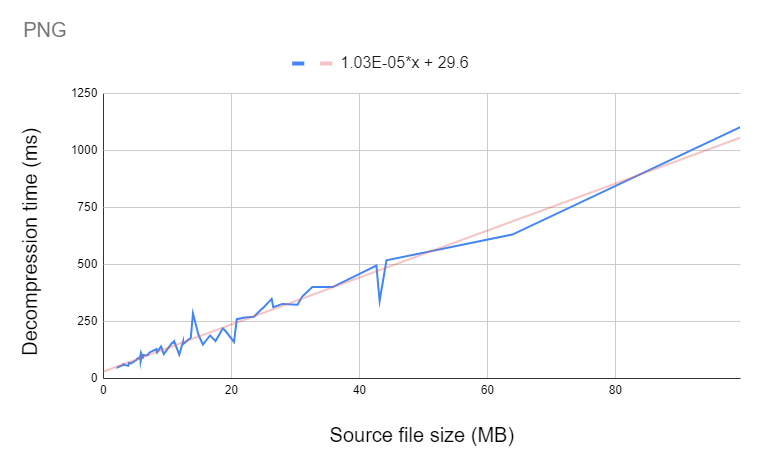
\includegraphics[width=0.475\textwidth]{OPNG.png}
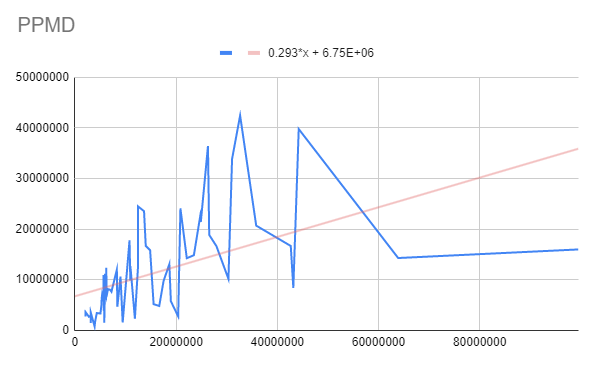
\includegraphics[width=0.475\textwidth]{OPPMD.png}
\caption{\label{fig:oPlot}Complexity graph. PNG (left) \& PPMd (right)}
\end{figure}

As can be seen, there is a sizable difference between algorithms in terms of their growth and stability. PNG on the left shows a linear growth relatively predictably. PPMd on the right, in comparison, shows a rather steep growth and appears to be fairly unpredictable. 

\subsection{Model}

Latency in formula \ref{networkfun}, as predicted by the complexity model in the previous section, can be substituted. This allows us to plot several graphs and draft a theoretical model to extrapolate this data to a broader spectrum of real world possibilities.

By applying both the complexity and network models the following formula can be derived:

\begin{equation}
T = (size_0 * ratio) / speed + size_0 * factor + base
\end{equation}

While this formula allows plotting a graph, it may be difficult to see any changes in performance. Performance is usually measured against the default value, in this case it is the value as described by formula \ref{networkfundefault}. Here, plots show the ratio of $T$ over its default counterpart.

Given a network speed of 650 KB/s, figure~\ref{fig:cNetwork-vSize-Ratio} shows the theoretical performance given a variable source file size. Given a source file of 5 MB, figure~\ref{fig:cSize-vNetwork-Ratio} shows the theoretical performance given a variable network speed.

\begin{figure}[!htb]
\centering
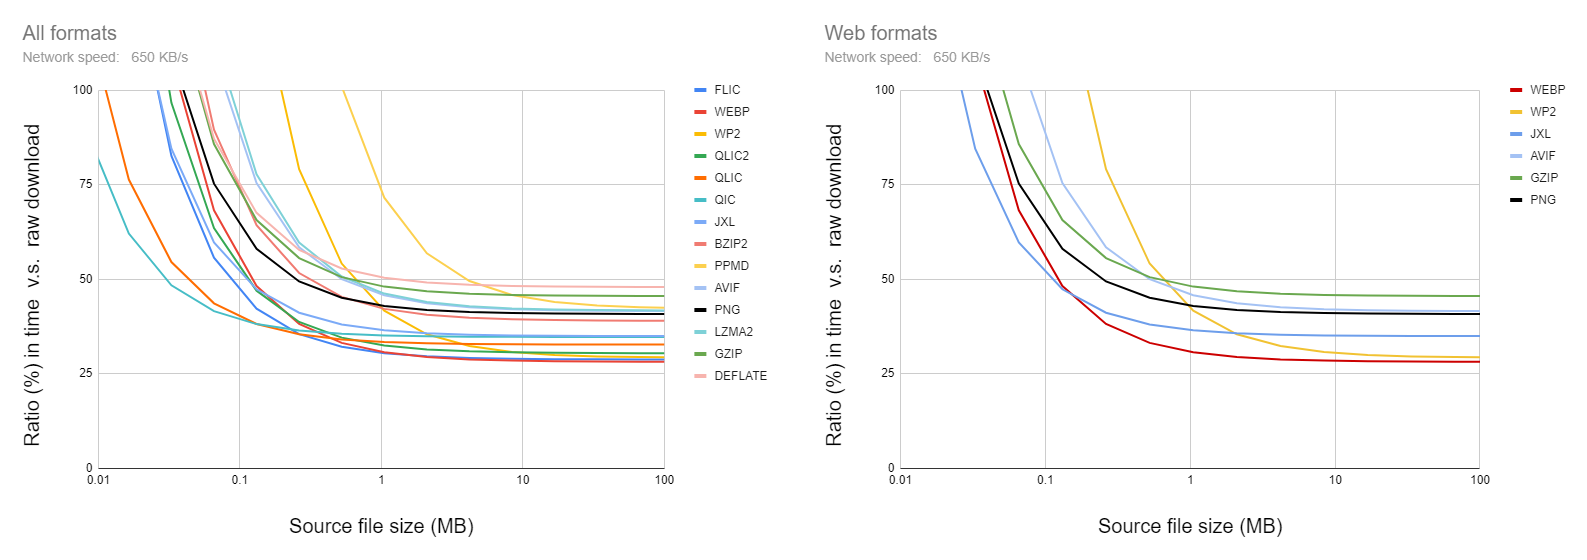
\includegraphics[width=1\textwidth]{cNetwork-vSize-Ratio.png}
\caption{\label{fig:cNetwork-vSize-Ratio} Performance model $\quad size \in \lbrack10KB, 100MB\rbrack \quad speed = 650KB/s$}
\end{figure}

\begin{figure}[!htb]
\centering
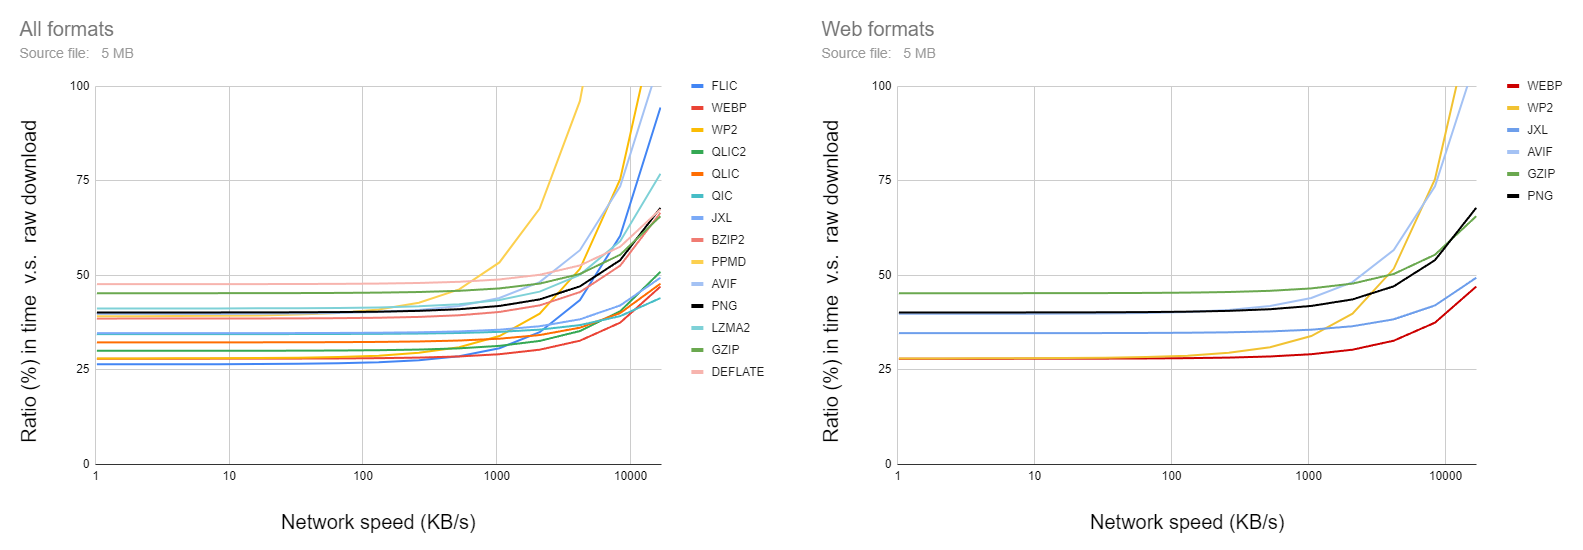
\includegraphics[width=1\textwidth]{cSize-vNetwork-Ratio.png}
\caption{\label{fig:cSize-vNetwork-Ratio} Performance model $\quad speed \in \lbrack 1KB/s, 1.7MB/s\rbrack \quad size = 5MB$}
\end{figure}

\newpage
\section{Real data}

\subsection{Measurements}

The model put forward in figure~\ref{fig:cNetwork-vSize-Ratio} is theoretical. The benchmark that has been conducted can also be plotted to the same graph. The measurement from a few algorithms are plotted in the following graph.

\begin{figure}[ht!]
\centering
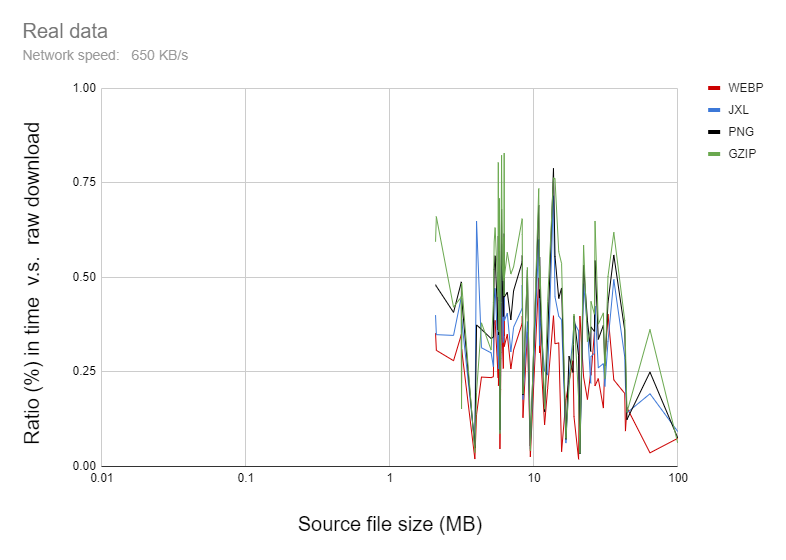
\includegraphics[width=0.8\textwidth]{cNetwork-vSize-Ratio-Real.png}
\caption{\label{fig:cNetwork-vSize-Ratio-Real} Real measurements}
\end{figure}

The first thing to note is that there is no data before a source file of a size smaller than about 2 MB. The reason for this is that no image tested in the benchmark is smaller than this. Secondly the performance is, as expected, heavily dependant on the image and great unpredictability can be noted. However, the plots seem to have a general relative order, WebP finds itself consistently below the others, whereas Gzip lags behind. This is in line with the theoretical model.

\newpage
\subsection{Ranking}

By averaging all this data out for every algorithm. The charts shown in figure~\ref{fig:Real} can be built up. Separate values are displayed for the download time, the former including decompression time, and the former including decompression time. The right chart in figure~\ref{fig:Real} shows common web formats only.

\begin{figure}[!htb]
\centering
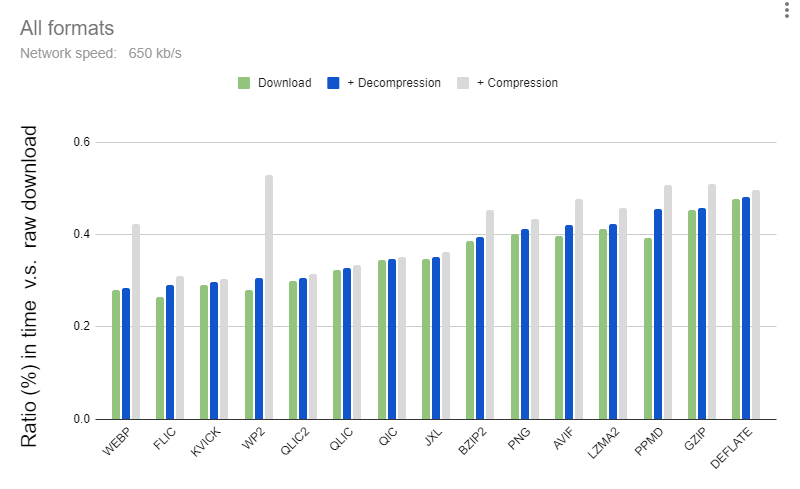
\includegraphics[width=0.8\textwidth]{Ratio-Real.png}
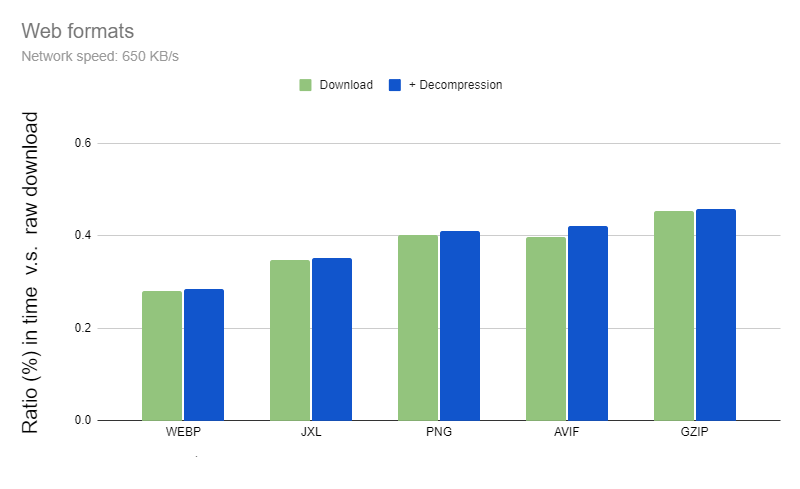
\includegraphics[width=0.8\textwidth]{Ratio-Real-Common.png}
\caption{\label{fig:Real} Ranking of formats}
\end{figure}

\newpage
\subsection{Effort}

The former testing data shows the result for the medium test conducted with a fixed effort level. Some algorithms allow higher effort levels and this may have effects on compression ratio and decompression time. Two values that influence their performance as measured in this paper. The plot in figure~\ref{fig:vEffort} shows the differences between effort levels for the algorithms that allow it.

The algorithms appear to gain performance when effort levels are increased. However, when compared to the growth in compression time this option becomes rather unappealing as seen in figure~\ref{fig:vEffortCompression}. Note the vertical axis is scaled logarithmically. In this small test, AVIF soared to a compression time of over 300 seconds at its peak. 

Disregarding compression times and solely focusing on download and decompression performance allows drafting update charts when applying the improvement measurements to figures \ref{fig:cNetwork-vSize-Ratio} and \ref{fig:cSize-vNetwork-Ratio}. For each algorithm, the maximum gain in effort is taken and applied the measured values. 

The same can be done for the real data in figure \ref{fig:Real} resulting in figure\ref{fig:vEffortReal}.

\begin{figure}[!htb]
\centering
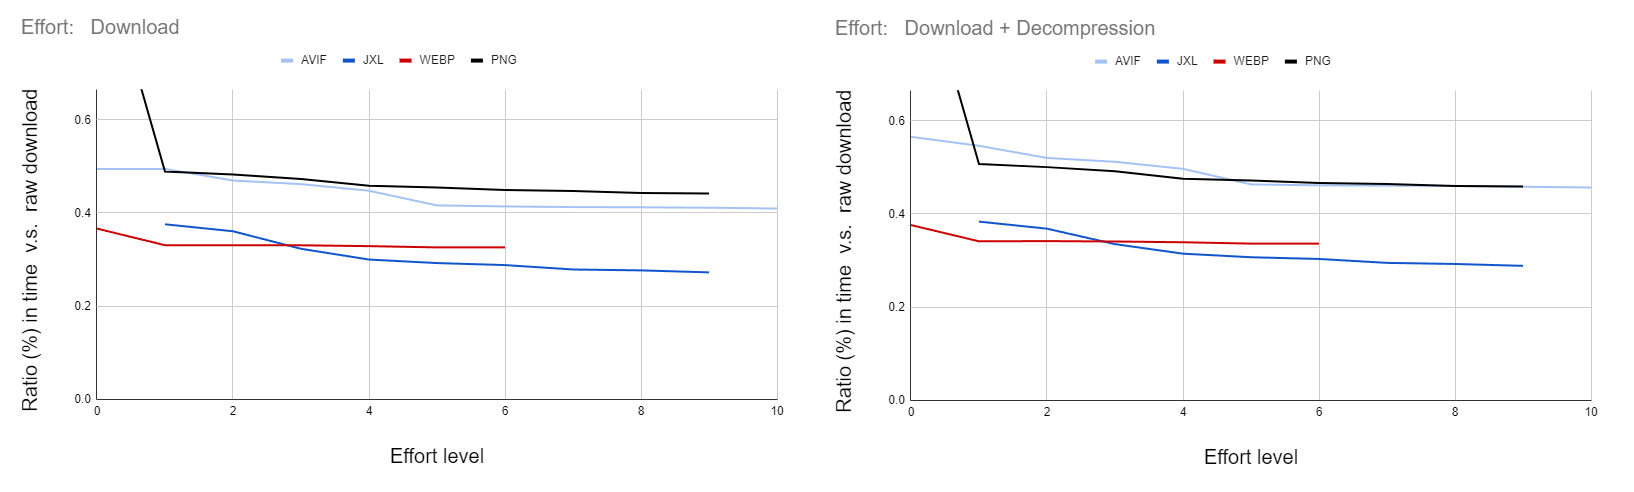
\includegraphics[width=1\textwidth]{vError-Real.png}
\caption{\label{fig:vEffort} Effects of effort}
\end{figure}

\begin{figure}[!htb]
\centering
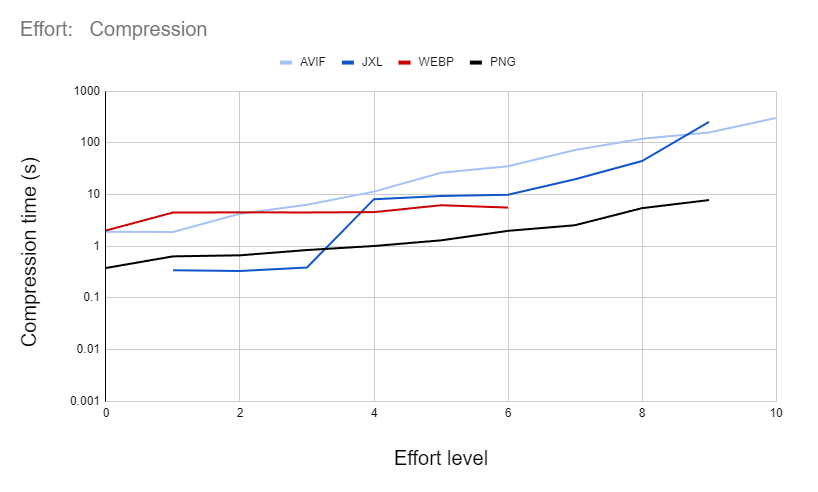
\includegraphics[width=0.5\textwidth]{vEffort-Real-Compression.png}
\caption{\label{fig:vEffortCompression} Effects of effort on compression time}
\end{figure}

%\begin{figure}[!htb]
%\centering
%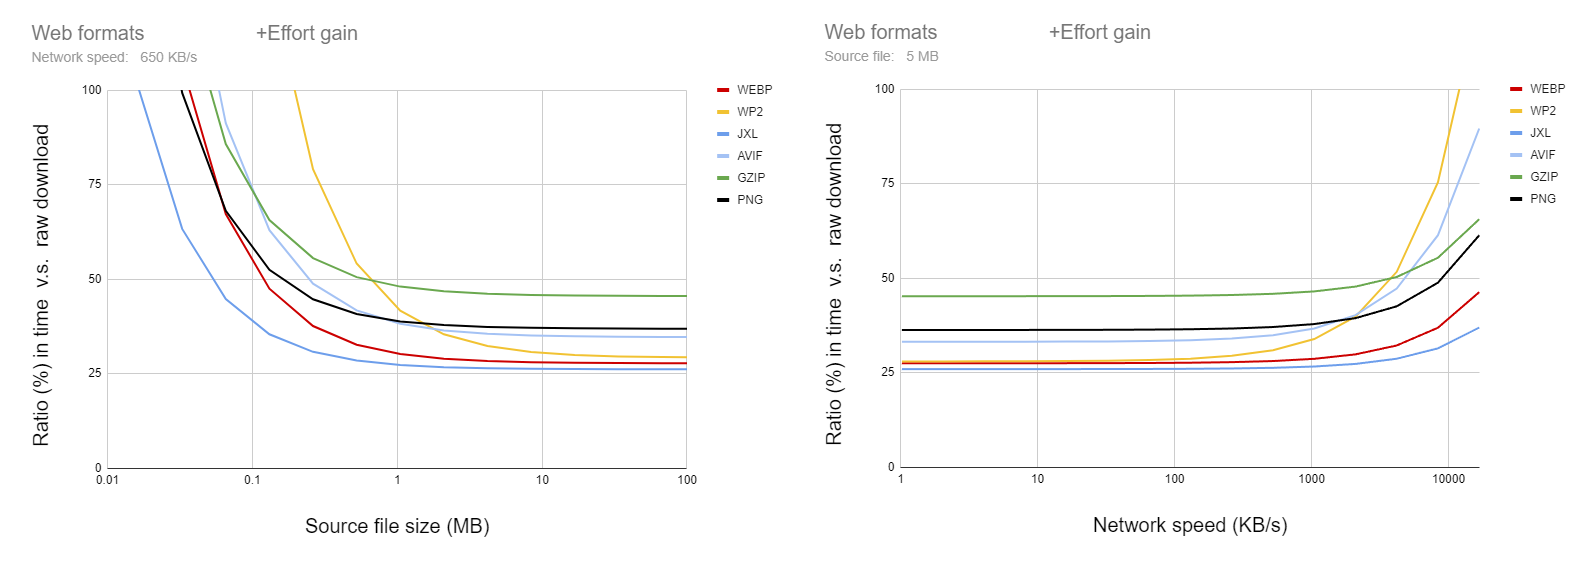
\includegraphics[width=1\textwidth]{vSize-vNetwork-Ratio-Effort.png}
%\caption{\label{fig:vEffortModel} Model graphs with additional effort gains}
%\end{figure}

\begin{figure}[!htb]
\centering
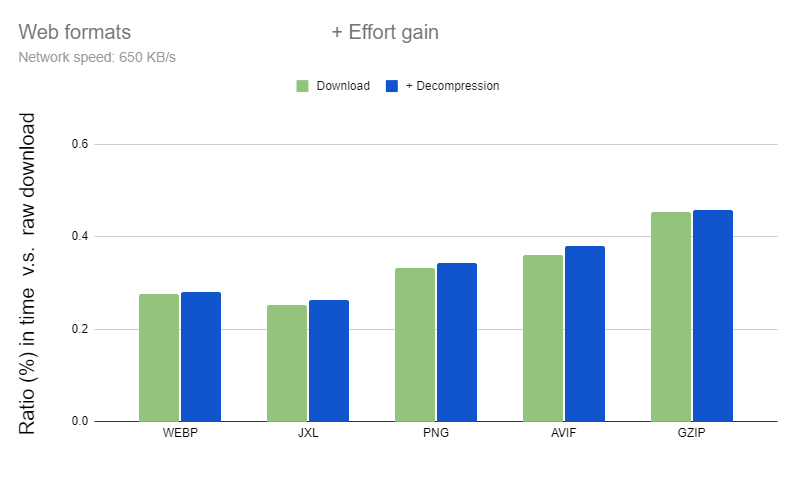
\includegraphics[width=0.8\textwidth]{Ratio-Real-Common-Effort.png}
\caption{\label{fig:vEffortReal} Real data with additional effort gains}
\end{figure}

\newpage

\chapter{Conclusion}

%Concluding the experiments, final statements can be put forward.

\section{Model}

The model put forward in \ref{analysis} were able to show interesting data. However, it has been shown by figure~\ref{fig:cNetwork-vSize-Ratio-Real} that this is a rather unreliable model. While not incorrect, the great discrepancies in real measurements given the same parameters tell that more and well tailored tests should be conducted to fit a use case.

\section{Real data}

A fair amount of testing data has been used to form the chart in figure~\ref{fig:Real}. This graph shows that WebP consistently performs well, together with the formats Flic and Kvick. Although Kvick had an error rate that was rather high this result cannot be taken as any conclusion. WebP 2 also performed well, falling just behind that of WebP. Since this format is still experimental this is all that can be said about it. Compression times were rather high for both WebP end WebP 2.

Jpeg XL can be found after the strong performers. When also accounting for effort as shown in figure~\ref{fig:vEffortReal}, Jpeg XL managed to become a strong competitor. In this whole study the winner in absolute terms. But as shown in figure~\ref{fig:vEffortCompression}, the compression time needed to achieve this performance is rather costly compared the the other options available.

The first general compression algorithm presents itself after Jpeg XL. PNG roughly shows the same performance as it implements a general compression algorithms as well, this result was to be expected.

AVIF appeared to not perform well in the tests performed. Why this is the case is uncertain. In the back the remaining general algorithms can be found. While still providing improvements over the default, they are as expected not optimal for images.

\newpage
\section{Conclusion}

\textbf{Jpeg XL} holds the winning title in this study. However, it requires a high level of effort to achieve this. \textbf{WebP} has shown balance and provides better performance where compression time is not unlimited. The most common lossless format, PNG, is shown to not be the optimal solution for a fast delivery of images. Furthermore, some niche formats have also shown competitive results.

\newpage
\pagenumbering{gobble}

\begin{thebibliography}{9}

\bibitem[Poskanzer \& Henderson. 2021]{ppm}
Poskanzer, J., Henderson, B. (2021). Netbpm. \textit{https://netpbm.sourceforge.net}

\bibitem[Leonard. 2016]{bmp}
Leonard, S. (2016). Windows Image Media Types. RFC 7903. \textit{10.17487/RFC7903}

\bibitem[CompuServe inc. 1987]{gif}
CompuServe inc. (1987). GIF (tm), Graphics Interchange Format. \textit{https://www.w3.org/Graphics/GIF/spec-gif87.txt}

\bibitem[Han et al. 2021]{av1spec}
Han, J., Li, B., Mukherjee, D., Chiang, C., Grange, A., Chen, C., Su, H., Parker, S., Deng, S., Joshi, U., Chen, Y., Wang, Y., Wilkins, P., Xu, Y. \& Bankoski, J. (2021). A Technical Overview of AV1. \textit{10.1109/JPROC.2021.3058584} 

\bibitem[W3 Consortium. 2022]{pngspec}
W3 Consortium (W3C). (2022). Portable Network Graphics (PNG) Specification (Third Edition). \textit{https://www.w3.org/TR/png/}

\bibitem[Rhatushnyak. 2022]{lpcb}
Rhatushnyak, A. (2022). Lossless Photo Compression Benchmark. \textit{http://qlic.altervista.org/LPCB.html}

\bibitem[Anonymous. 2020]{anonjxl}
Anonymous. (2020). Lossless Image Formats Comparison (Jpeg XL, AVIF, WebP 2, WebP, FLIF, PNG, ...) v1.27. \textit{https://docs.google.com/spreadsheets/d/1ju4q1WkaXT7WoxZINmQpf4ElgMD2VMlqeDN2DuZ6yJ8}

%\bibitem[Barina. 2021]{barinas}
%Barina, D. (2021). Comparison of Lossless Image Formats. \textit{https://arxiv.org/pdf/2108.02557.pdf}

\bibitem[Wikipedia. 2022]{streamalg}
Wikipedia. (2022). Streaming algorithm. Wikimedia Foundation. \textit{https://en.wikipedia.org/wiki/Streaming\_algorithm}

\bibitem[Mozilla Foundation. 2023]{browsersupport}
Mozilla Foundation. (2023). Image file type and format guide. The MDN Web Docs Project. \textit{https://developer.mozilla.org/docs/Web/Media/Formats/Image\_types}

\bibitem[Mozilla Foundation. 2022]{mozjpeg}
Mozilla Foundation. (2022). Improved JPEG encoder. \textit{https://github.com/mozilla/mozjpeg}

\bibitem[The libjpeg-turbo Project. 2022]{jpegturbo}
The libjpeg-turbo Project. (2022). SIMD-accelerated libjpeg-compatible JPEG codec library.
\textit{https://libjpeg-turbo.org}

\bibitem[Goolge  llc. 2022]{webp}
Google llc. (2022). WebP. An image format for the Web. \textit{https://developers.google.com/speed/webp}

\bibitem[Google llc. 2010]{webpstudy}
Goolge LLC. (2010). Comparative study of WebP, JPEG and JPEG 2000.
\textit{https://developers.google.com/speed/webp/docs/c\_study}

\bibitem[AOMedia. 2023]{avif}
Alliance for Open Media. (2023). libavif - Library for encoding and decoding .avif files. \textit{https://github.com/AOMediaCodec/libavif}

\bibitem[JPEG. 1992]{jpeg}
JPEG. (1992). Information technology — Digital compression and coding of continuous-tone still images \textit{ISO/IEC 10918}

\bibitem[MSU Media Group. 2020]{dcgc}
MSU Media Group. (2020). Data Compression Global Competition. Video Lab. Graphics and Media Lab. MSU Media group. Moscow State University. \textit{https://globalcompetition.compression.ru}

\bibitem[Pavlov. 2022]{7zip}
Pavlov, I. (2022). 7-Zip \& Lempel–Ziv–Markov chain algorithm (LZMA). \textit{https://www.7-zip.org}

\bibitem[Ziv \& Lempel. 1977]{LZ77}
Ziv, J., Lempel, A. (1977). A universal algorithm for sequential data compression. \textit{10.1109/TIT.1977.1055714}

\bibitem[Seward. 2019]{bzip2}
Seward, J. (2019). bzip2. \textit{https://sourceware.org/bzip2/}

\bibitem[Shkarin. 2003]{ppmd}
Shkarin, D. (2003). PPM: One step to practicality. Institute for Dynamics of Geospheres. \textit{https://compression.ru/compression.ru/ds/}. \textit{http://compression.graphicon.ru/download/articles/ppm/shkarin\_2002dcc\_ppmii\_pdf.rar}

\bibitem[FSF. 2020]{gzip}
Free Software Foundation. (2020). GNU Gzip. \textit{https://www.gnu.org/software/gzip/}

\bibitem[Google llc. 2022]{webp2}
Google llc. (2022). WebP 2: experimental successor of the WebP image format. Git repositories on chromium. \textit{https://chromium.googlesource.com/codecs/libwebp2/}

\bibitem[JPEG XL Project. 2022]{jxl}
JPEG XL Project. (2022). JPEG XL image format reference implementation. \textit{https://github.com/libjxl/libjxl}

\bibitem[ImageMagick Studio llc. 1999]{imagemagick}
ImageMagick Studio LLC. (1999). ImageMagick® is a free and open-source software suite for displaying, converting, and editing raster image and vector image files. \textit{https://imagemagick.org}

\bibitem[ISO/IEC JTC 1/SC 29. 2022]{jxlspec}
The Joint Photographic Experts Group (JPEG) committee (ISO/IEC JTC 1/SC 29/WG 1). (2022). Information technology — JPEG XL image coding system. \textit{ISO/IEC 18181}

\bibitem[Microsoft. 2022]{ps}
Microsoft. (2022). PowerShell. \textit{https://microsoft.com/powershell}

\bibitem[w77. 2022]{imdisk}
w77. (2022). ImDisk Toolkit: Ramdisk for Windows and mounting of image files. \textit{https://sourceforge.net/projects/imdisk-toolkit/}

\end{thebibliography}


\newpage
\pagenumbering{roman}

\appendix

\chapter{Artifatcs\label{app:repo}}

Vrijsen, K. (2023).

Image compression: On-demand systems seeking minimal latency.

\textit{https://git.konelinx.be/ImageCompressionODSSML} 

\textit{https://github.com/KoneLinx/ImageCompressionODSSML}

\chapter{Complexity graphs\label{app:ographs}}

\begin{figure}[ht!]
\centering
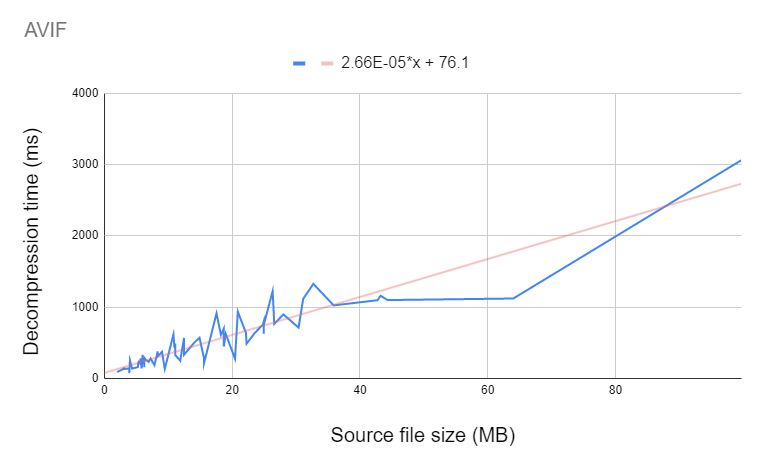
\includegraphics[width=0.475\textwidth]{OAVIF.png}
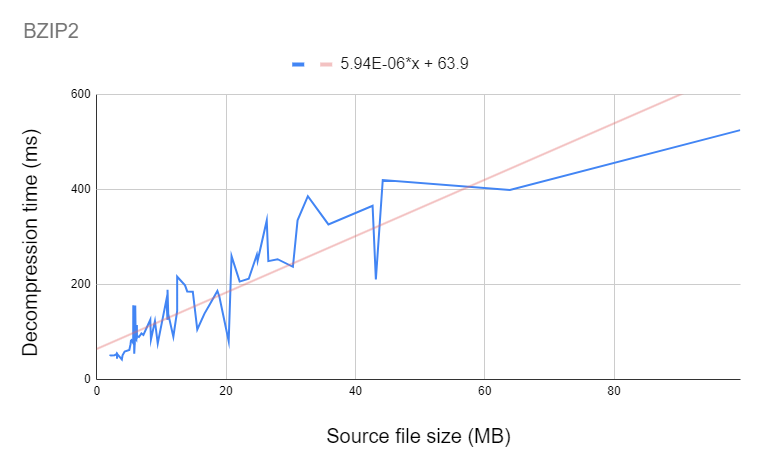
\includegraphics[width=0.475\textwidth]{OBZIP2.png}
\end{figure}

\begin{figure}[ht!]
\centering
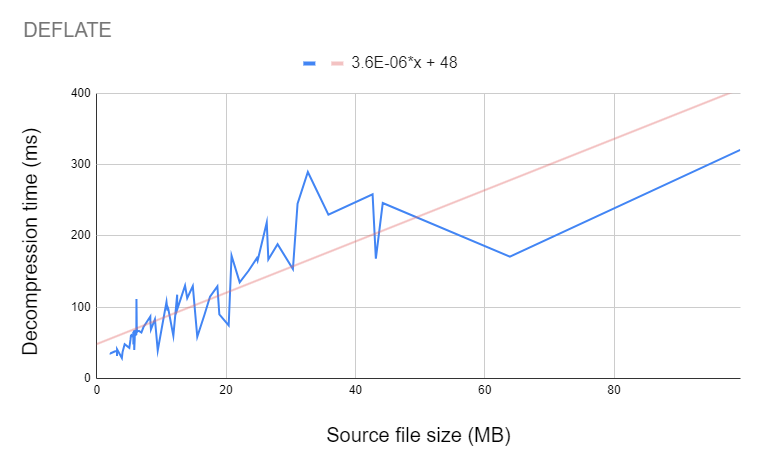
\includegraphics[width=0.475\textwidth]{ODEFLATE.png}
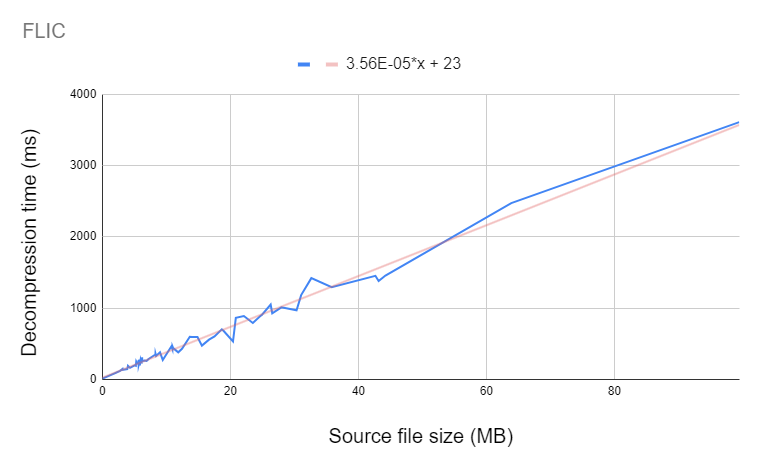
\includegraphics[width=0.475\textwidth]{OFLIC.png}
\end{figure}

\begin{figure}[ht!]
\centering
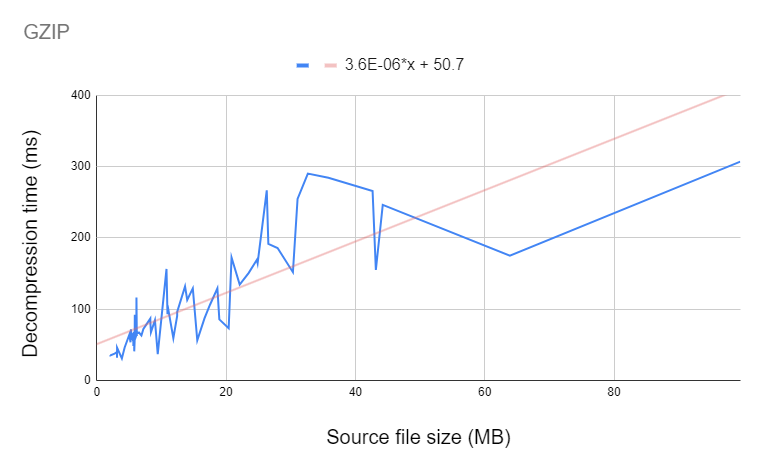
\includegraphics[width=0.475\textwidth]{OGZIP.png}
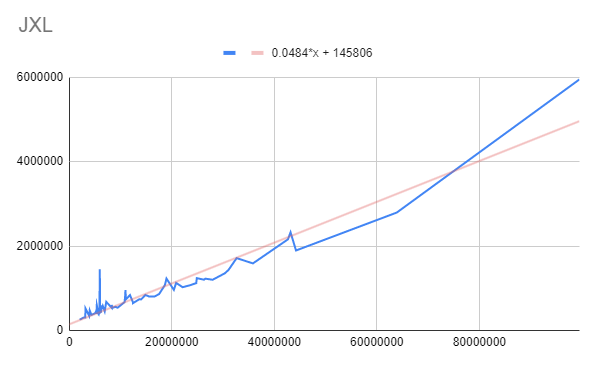
\includegraphics[width=0.475\textwidth]{OJXL.png}
\end{figure}

\begin{figure}[ht!]
\centering
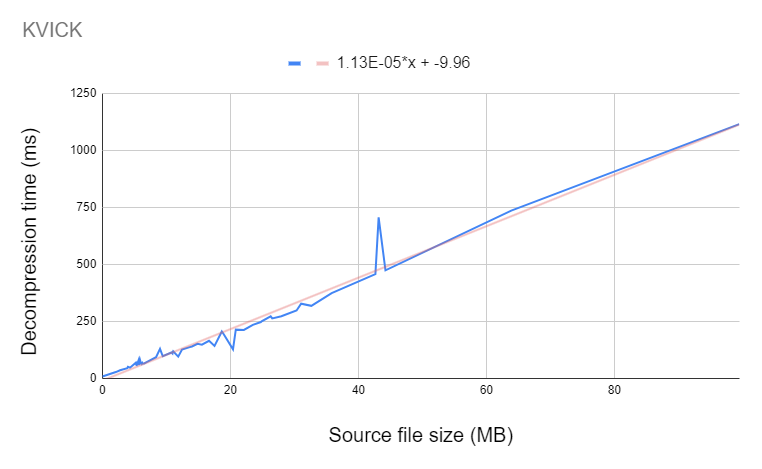
\includegraphics[width=0.475\textwidth]{OKVICK.png}
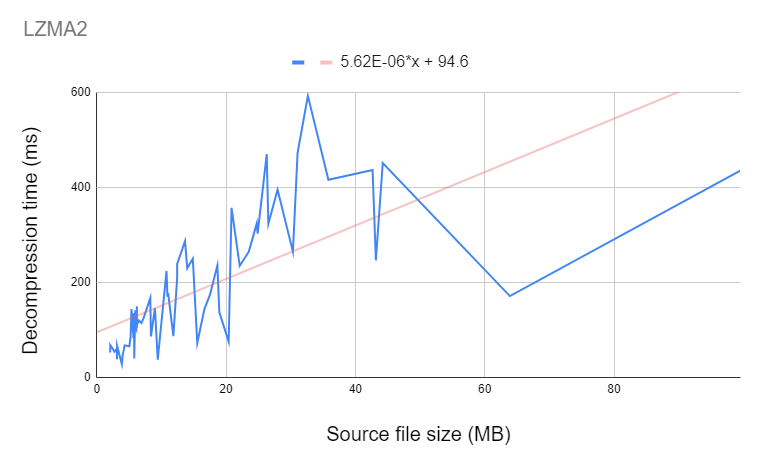
\includegraphics[width=0.475\textwidth]{OLZMA2.png}
\end{figure}

\begin{figure}[ht!]
\centering
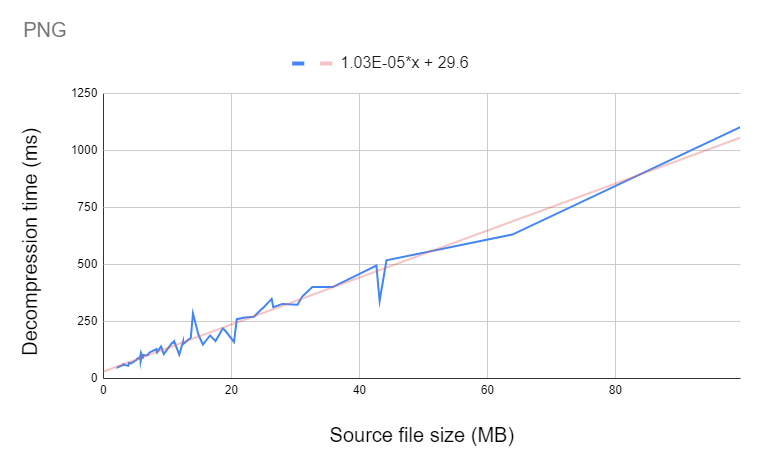
\includegraphics[width=0.475\textwidth]{OPNG.png}
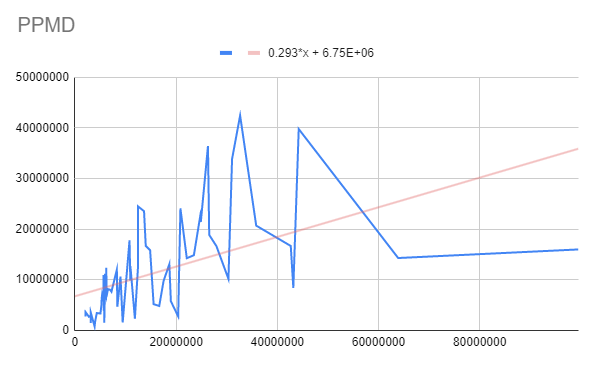
\includegraphics[width=0.475\textwidth]{OPPMD.png}
\end{figure}

\begin{figure}[ht!]
\centering
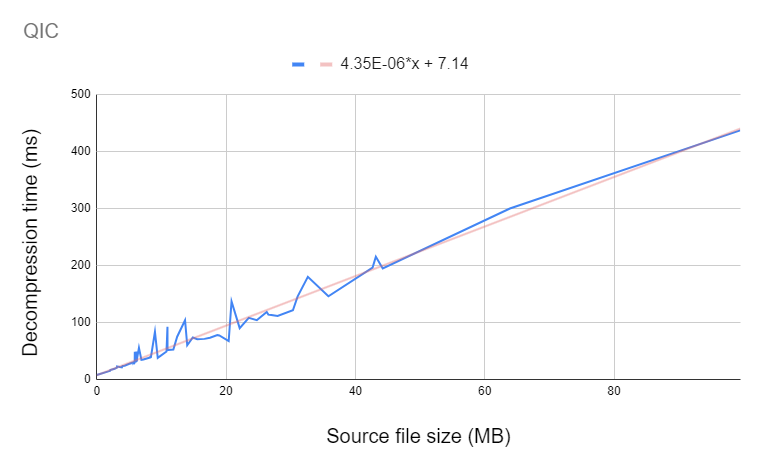
\includegraphics[width=0.475\textwidth]{OQIC.png}
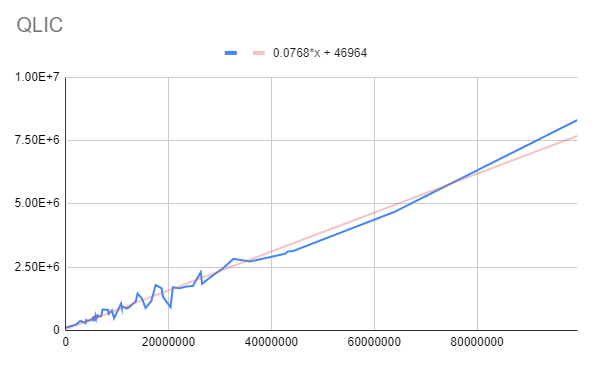
\includegraphics[width=0.475\textwidth]{OQLIC.png}
\end{figure}

\begin{figure}[ht!]
\centering
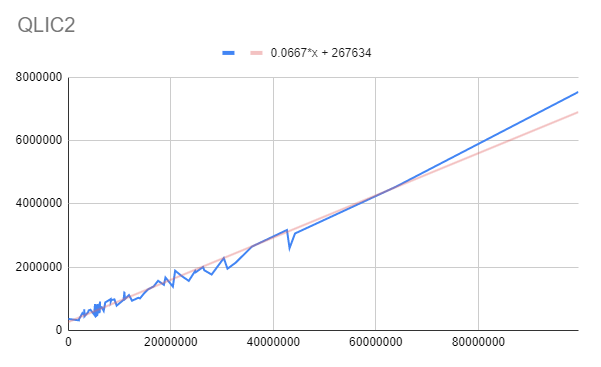
\includegraphics[width=0.475\textwidth]{OQLIC2.png}
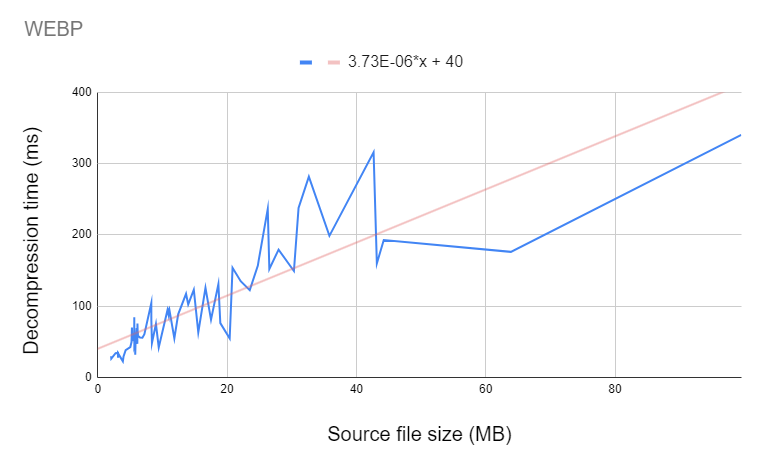
\includegraphics[width=0.475\textwidth]{OWEBP.png}
\end{figure}

\begin{figure}[ht!]
\centering
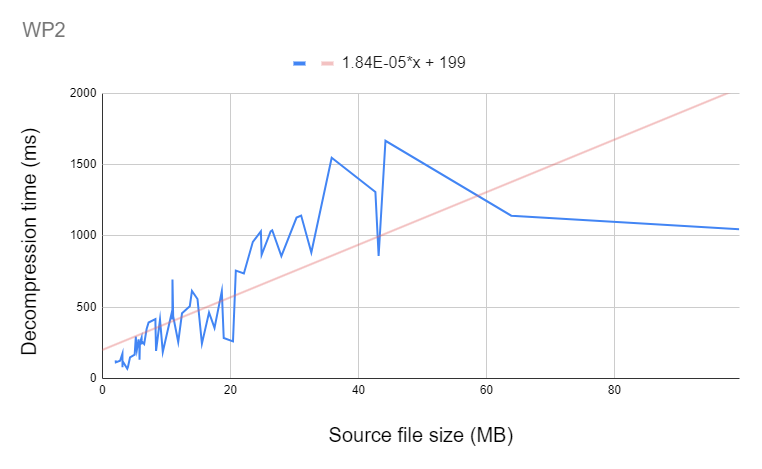
\includegraphics[width=0.475\textwidth]{OWP2.png}
\end{figure}

\chapter{Models\label{app:models}}

\begin{figure}[ht!]
\centering
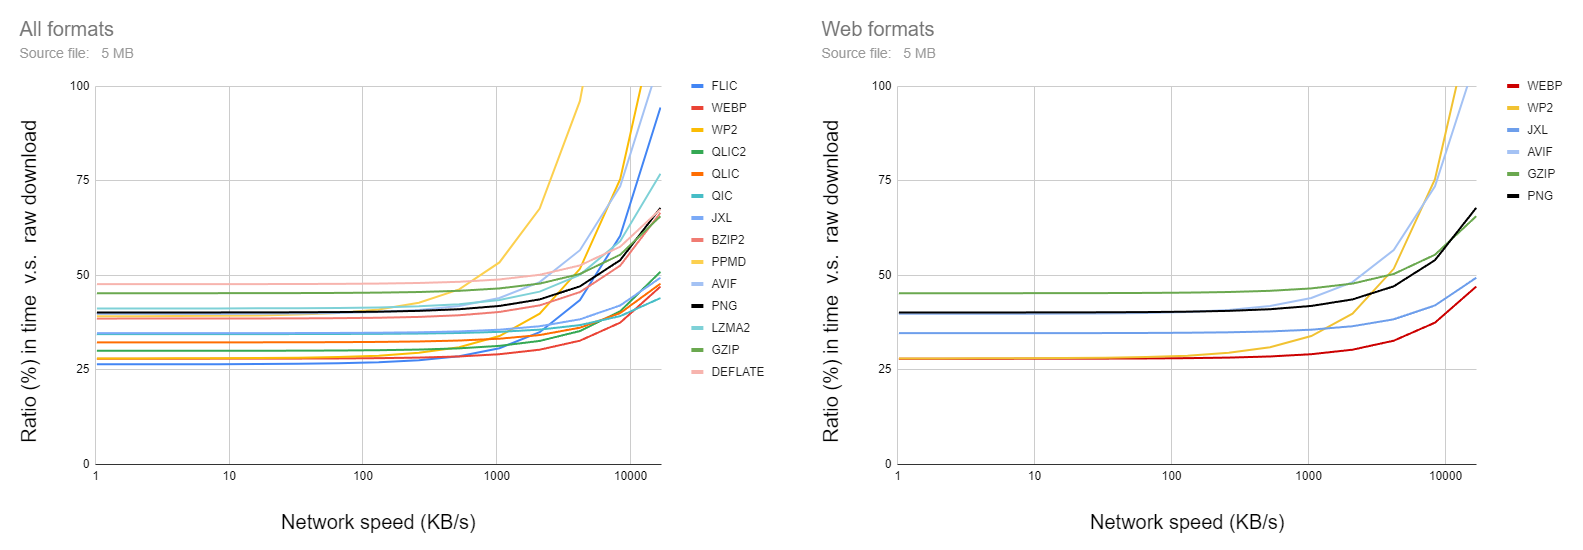
\includegraphics[width=1\textwidth]{cSize-vNetwork-Ratio.png}
\end{figure}

\begin{figure}[ht!]
\centering
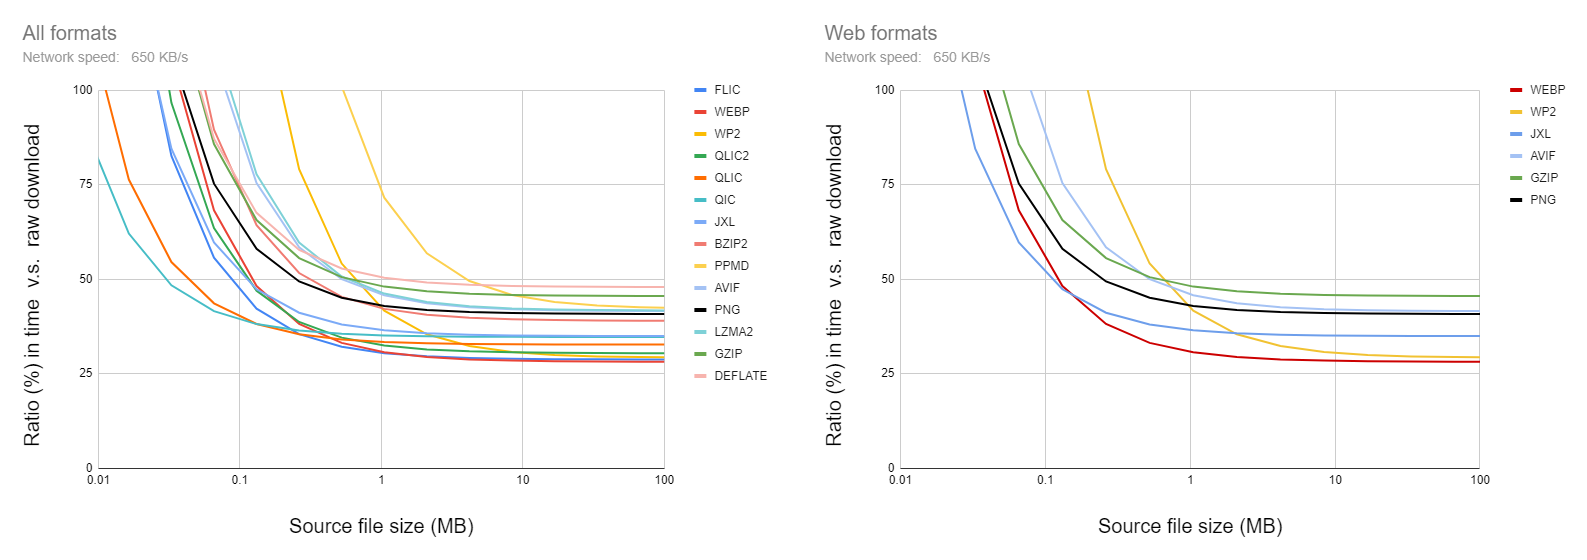
\includegraphics[width=1\textwidth]{cNetwork-vSize-Ratio.png}
\end{figure}

\begin{figure}[ht!]
\centering
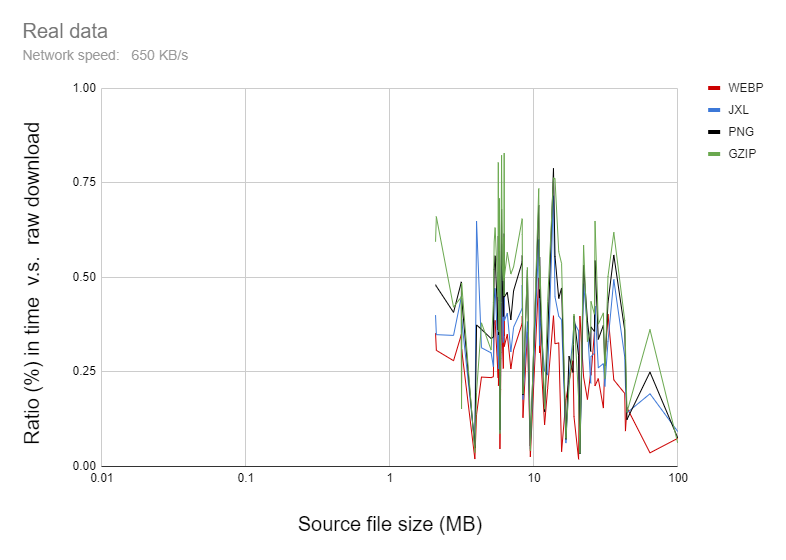
\includegraphics[width=0.8\textwidth]{cNetwork-vSize-Ratio-Real.png}
\end{figure}

\begin{figure}[ht!]
\centering
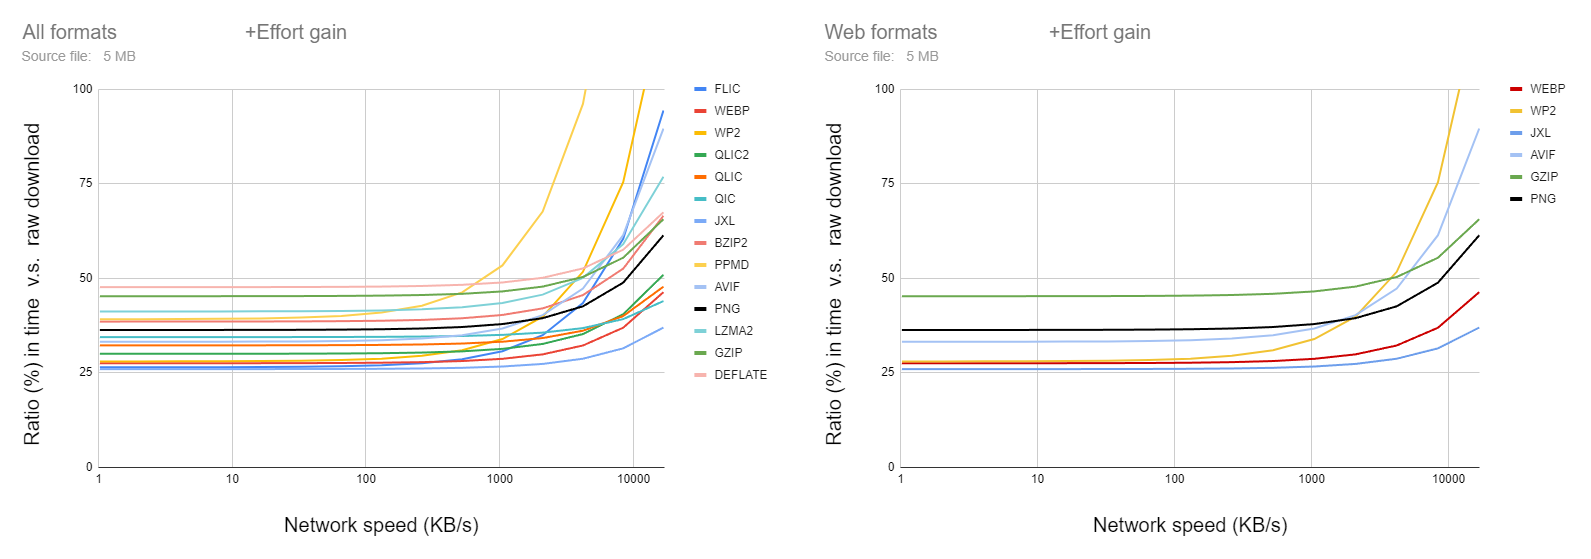
\includegraphics[width=1\textwidth]{cSize-vNetwork-Ratio-Effort.png}
\end{figure}

\begin{figure}[ht!]
\centering
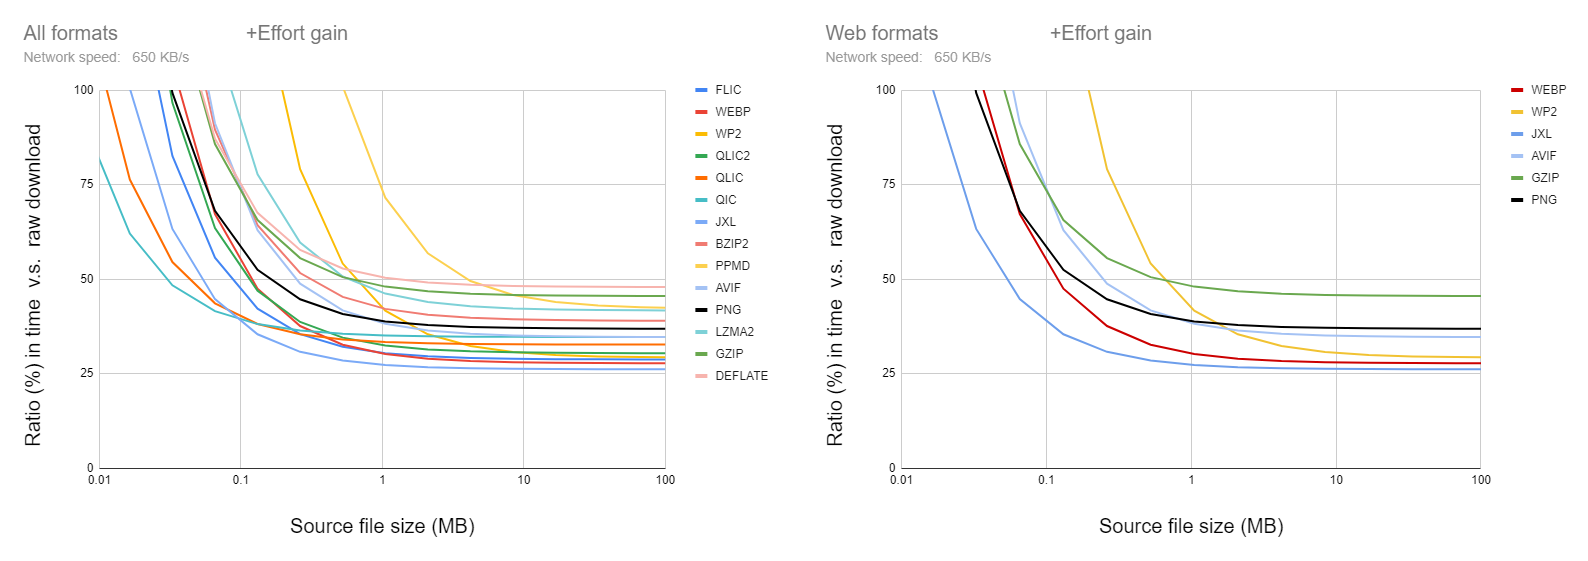
\includegraphics[width=1\textwidth]{cNetwork-vSize-Ratio-Effort.png}
\end{figure}

\chapter{Ranking\label{app:ranks}}

\begin{figure}[ht!]
\centering
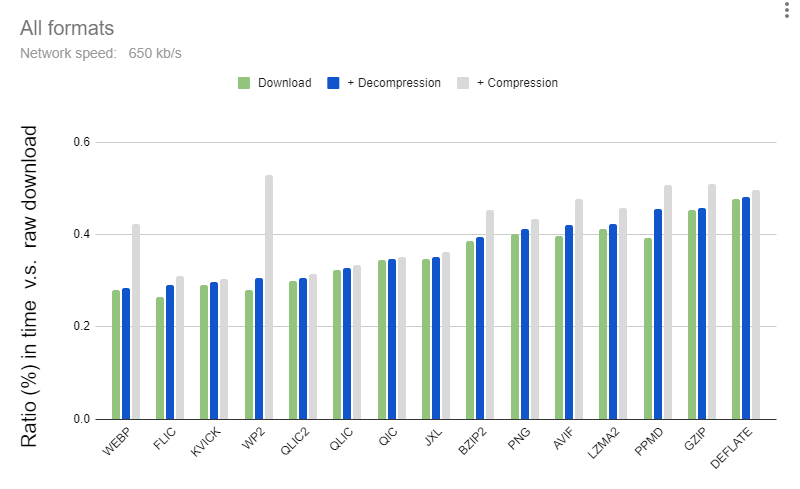
\includegraphics[width=1\textwidth]{Ratio-Real.png}
\end{figure}

\begin{figure}[ht!]
\centering
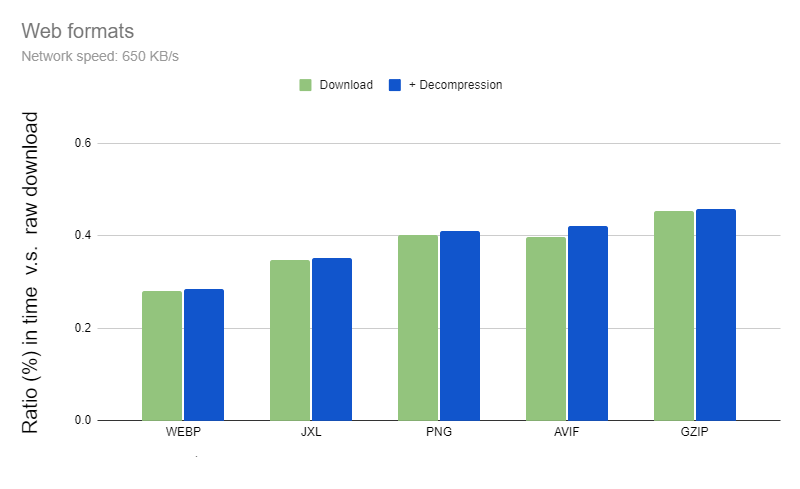
\includegraphics[width=1\textwidth]{Ratio-Real-Common.png}
\end{figure}

\begin{figure}[ht!]
\centering
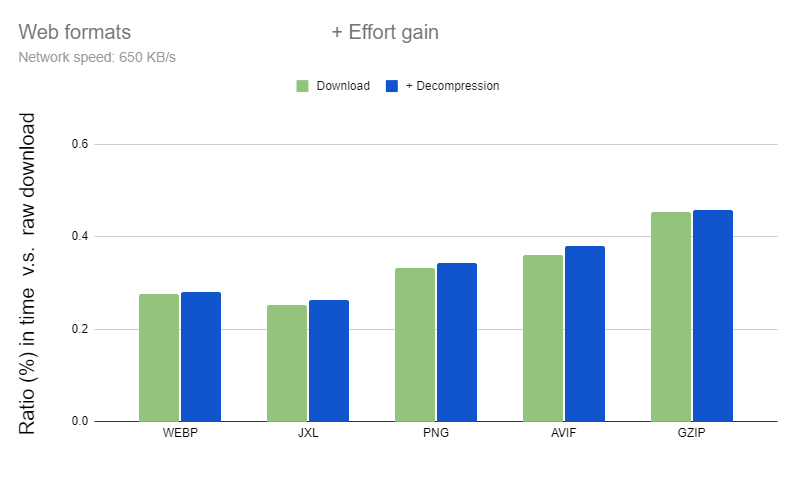
\includegraphics[width=1\textwidth]{Ratio-Real-Common-Effort.png}
\end{figure}

\chapter{Scripts\label{app:script}}

\definecolor{codegreen}{rgb}{0,0.45,0}
\definecolor{codeorange}{rgb}{0.35,0.35,0}
\definecolor{codeblue}{rgb}{0,0,0.89}
\definecolor{codegrey}{rgb}{0.45,0.45,0.45}
\lstdefinestyle{cmdstyle}{
    commentstyle=\color{codegreen},
    stringstyle=\color{codeorange},
    keywordstyle=\color{codeblue},
    tabsize=1,
    breaklines=true,
    basicstyle=\tiny\ttfamily\bfseries
}
\lstset{style=cmdstyle}
\lstinputlisting[language=sh]{BenchmarkExport2.ps1}

\newpage
\pagenumbering{gobble}

\begin{figure}
    \centering
\begin{center}
\item \textbf{Kobe Vrijsen}
\item \today
\item 
\item \textit{kobevrijsen@posteo.be}
\item \textit{konelinx.be}
\item 
\item CC BY 4.0 or above
\end{center}

\end{figure}

\end{document}
